\documentclass[11pt]{article}
\usepackage[margin=1in]{geometry}
\usepackage{amsmath, amssymb}
\usepackage{graphicx}
\usepackage{float}

\title{Project 1.5: From the Normal Distribution to $\chi^2$, $t$, and $F$}
\author{Matthew Hermosura, Zane Kelly, Jacob Le \\ STAT 4360}
\date{\today}

% Placeholder box for comments: replace the text inside \comment{...} with your own
\newcommand{\comment}[1]{\par\noindent\textbf{Comment:} #1\par\medskip}

\begin{document}
\maketitle

All simulations use $M = 5{,}000$ Monte Carlo replications and a fixed random
seed. Each figure shows a density-normalized histogram of the simulated values
with the theoretical density overlaid in red.

%==========================================================
\section*{Part 1: Simulating $\chi^2$, $t$, and $F$ from normal building blocks}

\subsection*{1.1 Chi-square ($n = 15$)}
$W = \sum_{i=1}^{15} Z_i^2$ with $Z_i \overset{iid}{\sim} N(0,1)$.

\begin{figure}[H]
  \centering
  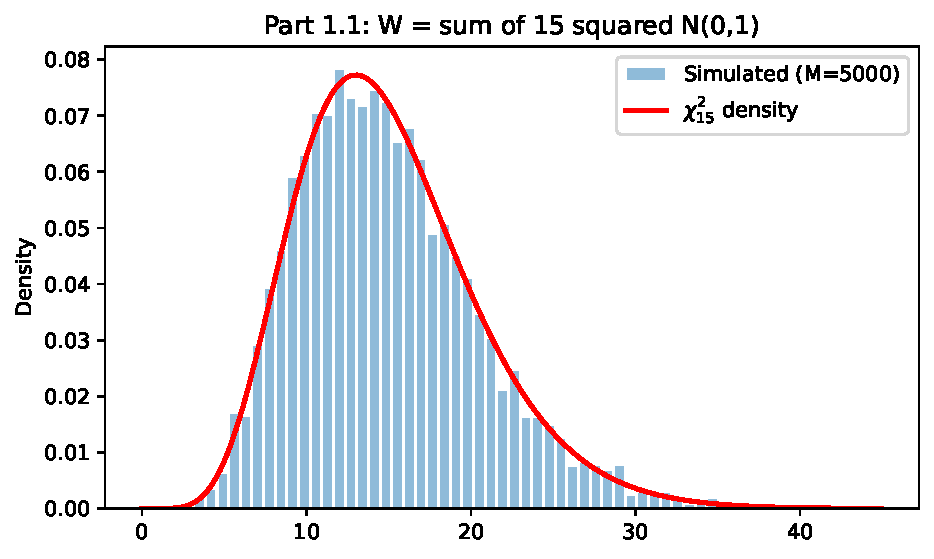
\includegraphics[width=0.75\textwidth]{figures/part1_1_chisq.pdf}
  \caption{Simulated $W$ vs.\ the $\chi^2_{15}$ density.}
\end{figure}

\comment{% Comment on the fit in one or two sentences.
The histogram follows the $\chi^2_{15}$ density closely: both are right-skewed
with a peak near 13 and a long right tail. The simulated mean and variance
(15.00 and 31.3) are close to the theoretical values $E(W) = n = 15$ and
$\operatorname{Var}(W) = 2n = 30$.
}

\subsection*{1.2 $t$ distribution ($n = 15$)}
$T = Z / \sqrt{V/15}$ with $Z \sim N(0,1)$ independent of $V \sim \chi^2_{15}$.

\begin{figure}[H]
  \centering
  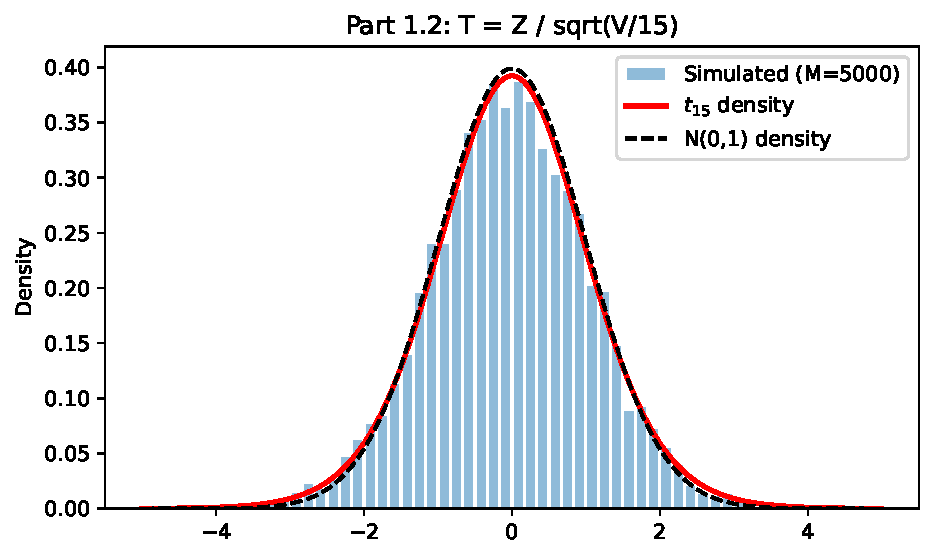
\includegraphics[width=0.75\textwidth]{figures/part1_2_t.pdf}
  \caption{Simulated $T$ vs.\ the $t_{15}$ density, with the $N(0,1)$ density (dashed) for comparison.}
\end{figure}

\comment{% How do the tails compare to the standard normal?
The histogram matches the $t_{15}$ density well. Compared with $N(0,1)$, the
$t_{15}$ curve has a slightly lower peak and slightly heavier tails, because
dividing by the random quantity $\sqrt{V/15}$ adds extra variability. The
difference is small at 15 degrees of freedom but shows up in the tails:
$|T| > 3$ occurred in 0.92\% of the simulated values, close to the $t_{15}$
probability of 0.90\% and more than three times the normal probability of 0.27\%.
}

\subsection*{1.3 $F$ distribution ($n_1 = 8$, $n_2 = 20$)}
$F = (U/8)/(V/20)$ with $U \sim \chi^2_8$ independent of $V \sim \chi^2_{20}$.

\begin{figure}[H]
  \centering
  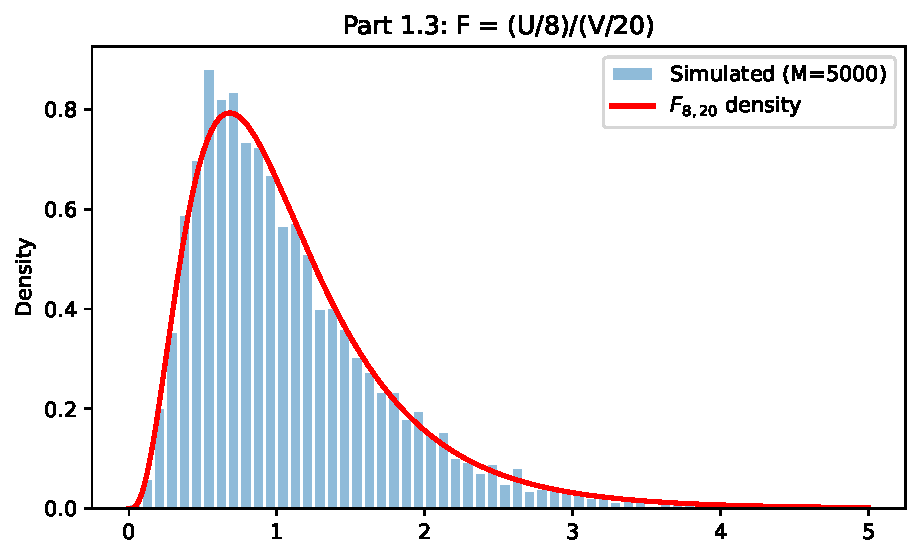
\includegraphics[width=0.75\textwidth]{figures/part1_3_F.pdf}
  \caption{Simulated $F$ vs.\ the $F_{8,20}$ density.}
\end{figure}

\comment{% Comment on the fit.
The histogram follows the $F_{8,20}$ density: it is strictly positive, peaks
below 1 (around 0.7), and has a long right tail. The simulated mean of 1.10 is
close to the theoretical mean $n_2/(n_2 - 2) = 20/18 \approx 1.11$.
}

%==========================================================
\section*{Part 2: What happens with a real sample}
$n = 20$, $\mu = 5$, $\sigma = 2$. Each repetition draws one sample
$X_1,\dots,X_n \overset{iid}{\sim} N(\mu,\sigma^2)$ and computes
\[
W' = \frac{(n-1)S^2}{\sigma^2}, \qquad T' = \frac{\sqrt{n}\,(\bar X - \mu)}{S}.
\]

\subsection*{$W'$ vs.\ $\chi^2_{n-1}$}
\begin{figure}[H]
  \centering
  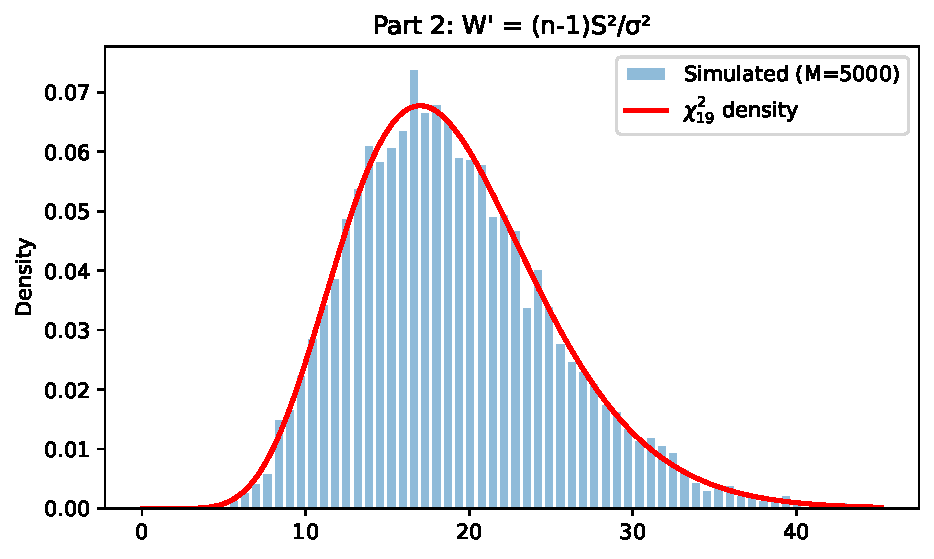
\includegraphics[width=0.75\textwidth]{figures/part2_W_prime.pdf}
  \caption{Simulated $W'$ vs.\ the $\chi^2_{19}$ density.}
\end{figure}

\comment{% Compare to the Part 1.1 plot: same shape? degrees of freedom relative to sample size?
$W'$ fits the $\chi^2_{19}$ density closely and has the same right-skewed shape
as the Part 1.1 plot, shifted right because it has more degrees of freedom. The
key difference is the relationship to sample size: in Part 1.1, summing
$n = 15$ squared normals gave $\chi^2_{15}$ (degrees of freedom $= n$), while here
a sample of $n = 20$ gives $\chi^2_{19}$ (degrees of freedom $= n - 1$). The
simulated mean of 19.05 matches 19, not 20.
}

\subsection*{$T'$ vs.\ $t_{n-1}$}
\begin{figure}[H]
  \centering
  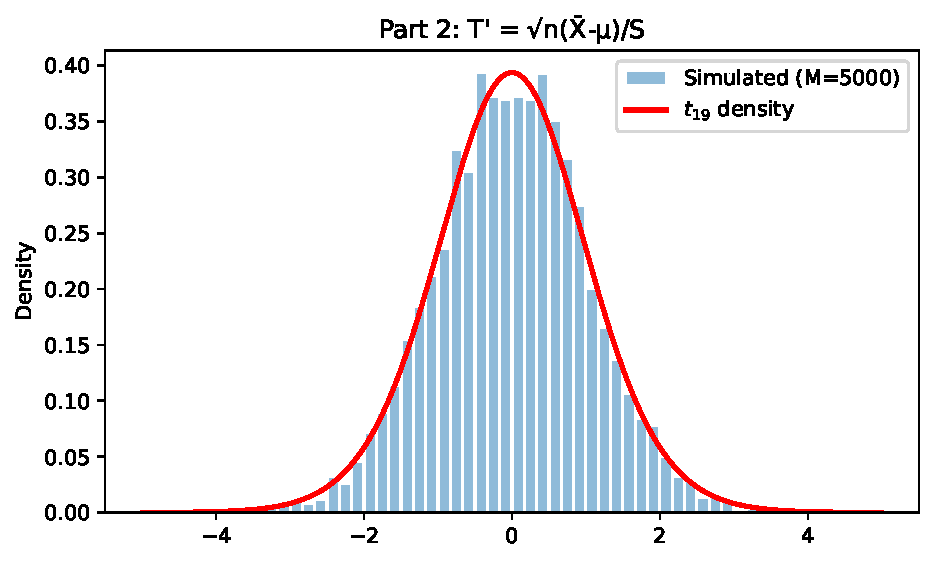
\includegraphics[width=0.75\textwidth]{figures/part2_T_prime.pdf}
  \caption{Simulated $T'$ vs.\ the $t_{19}$ density.}
\end{figure}

\comment{% Compare to the Part 1.2 plot.
$T'$ fits the $t_{19}$ density well and looks like the Part 1.2 plot: symmetric,
bell-shaped, and centered at 0. Even though $T'$ was computed from a single
sample with the unknown $\sigma$ replaced by $S$, it behaves exactly like a $t$
variable built from separate normals, with $n - 1 = 19$ degrees of freedom.
With more degrees of freedom than in Part 1.2, it is even closer to $N(0,1)$.
}

\subsection*{Why $n-1$ degrees of freedom?}
\comment{% 2-3 sentences: how many deviations X_i - Xbar are free to vary once Xbar is fixed?
$S^2$ is built from the deviations $X_i - \bar X$, and $\bar X$ is computed from
the same data, so these deviations must satisfy $\sum_{i=1}^n (X_i - \bar X) = 0$.
Once any $n - 1$ of them are known, the last one is determined, so only $n - 1$
of the deviations are free to vary. Estimating $\bar X$ therefore uses up one
degree of freedom, and $W'$ has $n - 1$ degrees of freedom instead of $n$.
}

%==========================================================
\section*{Part 3.1: Two samples, $F_{n_1-1,\,n_2-1}$}
$n_1 = 16$, $n_2 = 21$, $\mu_1 = 3$, $\mu_2 = -2$, $\sigma_1 = 2$, $\sigma_2 = 3$.
\[
F' = \frac{S_1^2/\sigma_1^2}{S_2^2/\sigma_2^2}.
\]

\begin{figure}[H]
  \centering
  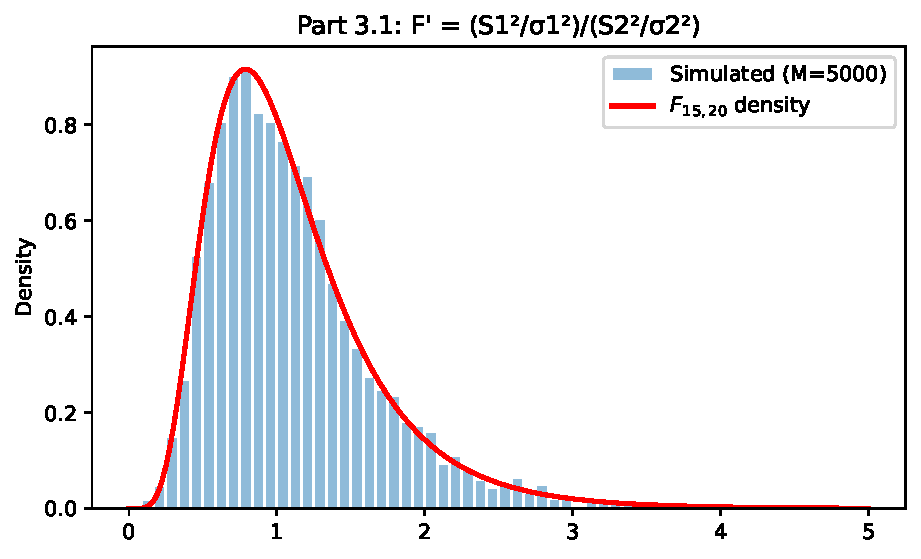
\includegraphics[width=0.75\textwidth]{figures/part3_1_F_prime.pdf}
  \caption{Simulated $F'$ vs.\ the $F_{15,20}$ density.}
\end{figure}

\comment{% Compare to the Part 1.3 plot.
$F'$ fits the $F_{15,20}$ density well and has the same positive, right-skewed
shape as the Part 1.3 plot. With more numerator degrees of freedom (15 instead
of 8), it is more concentrated, with a taller peak closer to 1. The simulated
mean of 1.12 is close to $20/18 \approx 1.11$. The different means
$\mu_1 = 3$ and $\mu_2 = -2$ have no effect, because sample variances do not
depend on where the data are centered.
}

\subsection*{Why $n_1 - 1$ and $n_2 - 1$?}
\comment{% 1-2 sentences.
Each sample variance is computed around its own sample mean, so each sample
loses one degree of freedom: $(n_1 - 1)S_1^2/\sigma_1^2 \sim \chi^2_{n_1 - 1}$ and
$(n_2 - 1)S_2^2/\sigma_2^2 \sim \chi^2_{n_2 - 1}$. Their ratio, each divided by
its degrees of freedom, is therefore $F_{n_1 - 1,\, n_2 - 1}$.
}

\end{document}
